\documentclass{article}
%% PACKAGES %%

\usepackage{amsmath, amsfonts, amssymb, amsthm}
\usepackage{braket}
\usepackage{listings}
\usepackage{geometry}
\usepackage{xcolor}
\usepackage{textcomp}
\usepackage{graphicx}
\usepackage{fancyhdr}
\usepackage{sourcecodepro}
\usepackage{multirow}

%%%%%%%%%%%%%%

\graphicspath{{./images}}
\setlength\parindent{0pt}       % globally supress indentation

%% LISTINGS CONFIG %%

\definecolor{purple2}{RGB}{153,0,153} % there's actually no standard purple
\definecolor{green2}{RGB}{0,153,0} % a darker green

\lstset{
  language=Verilog,                   % the language
  basicstyle=\normalsize\ttfamily,   % size of the fonts for the code
  frame = single,
  % Color settings to match IDLE style
  keywordstyle=\color{orange},       % core keywords
  keywordstyle={[2]\color{purple2}}, % built-ins
  stringstyle=\color{green2},%
  showstringspaces=false,
  commentstyle=\color{red},%
  upquote=true,                      % requires textcomp
  numbers=left,
  breaklines=true,
}

% Title Stuff
\title{\vspace{-3cm} ECE426 HW7 \\ \textit{\normalsize ROM Signed Multiplication}}
\author{Chase A. Lotito, \textit{SIUC Undergraduate}}
\date{}

\begin{document}

\pagestyle{fancy}

% attempt to make nice header
\fancyhead{}
\fancyhead[CH]{\normalsize{LOTITO - SIUC ECE - SPRING 2024}}

\maketitle % Makes the title

\section*{Question}

A ROM can be used to multiply two binary numbers by splitting the address lines to accommodate the two numbers. Implement using Verilog such as a multiplier for multiplying two signed numbers, each of size 4 bits.

\bigskip

\textbf{Part A.}

The solution code is provided below.

\begin{lstlisting}
// Chase Lotito - SIUC - Spring 2024
// ECE426 - HW7

module rom (n1, n2, result);

input [3:0] n1 ; // first signed Number
input [3:0] n2 ; // second signed Number
output [7:0] result ; // Result = n1 x n2.
wire [7:0] result ;
wire [3:0] n1_mag ;
wire [3:0] n2_mag ;
reg [7:0] product ;

// converting from 2's comp
// gameplan:
//  - check if positive
//      - if yes, just assign
//      - if no, find twos complement
assign n1_mag = (n1[3] == 0) ? n1 : (~n1 + 1); // get magnitude of n1
assign n2_mag = (n2[3] == 0) ? n2 : (~n2 + 1); // get magnitude of n2

always @ (n1_mag or n2_mag) begin
    case ({n1_mag, n2_mag})
        // 1 * n2_mag
        17 : product = 1;
        18 : product = 2;
        19 : product = 3;
        20 : product = 4;
        21 : product = 5;
        22 : product = 6;
        23 : product = 7;
        24 : product = 8;
        // 2 * n2_mag
        33: product = 2;
        34: product = 4;
        35: product =  6;
        36: product =  8;
        37: product =  10;
        38: product =  12;
        39: product =  14;
        40: product =  16;
        // 3 * n2_mag
        49: product = 3;
        50: product = 6;
        51: product = 9;
        52: product = 12;
        53: product = 15;
        54: product = 18;
        55: product = 21;
        56: product = 24;
        // 4 * n2_mag
        65: product = 4;
        66: product = 8;
        67: product = 12;
        68: product = 16;
        69: product = 20;
        70: product = 24;
        71: product = 28;
        72: product = 32;
        // 5 * n2_mag
        81 : product = 5;
        82: product = 10;
        83: product = 15;
        84: product = 20;
        85: product = 25;
        86: product = 30;
        87: product = 35;
        88: product = 40;
        // 6 * n2_mag
        97 : product = 6;
        98: product = 12;
        99: product = 18;
        100: product = 24;
        101: product = 30;
        102: product = 36;
        103: product = 42;
        104: product = 48;
        // 7 * n2_mag
        113: product = 7;
        114: product = 14;
        115: product = 21;
        116: product = 28;
        117: product = 35;
        118: product = 42;
        119: product = 49;
        120: product = 56;
        // 8 * n2_mag
        129: product = 8;
        130: product = 16;
        131: product = 24;
        132: product = 32;
        133: product = 40;
        134: product = 48;
        135: product = 56;
        136: product = 64;
        default : product = 0 ; // Clear the result.
    endcase
end

// check if result should be signed or not via xnor
// if + then give positive product
// if - then give negative product
assign result = (~(n1[3] == 1 ^ n2[3] == 1)) ? product : (~product + 1);

endmodule
\end{lstlisting}

The testbench.

\begin{lstlisting}
// Chase Lotito - HW7 Testbench

`timescale 1ns / 1ns
`include "q1.v"

module tb();
 
initial begin
    $dumpfile("tb.vcd");
    $dumpvars(0, tb);
end

// I/O
reg [3:0] n1, n2;
wire [7:0] result;
reg [8:0] invect;

// Start-up procedures:
initial begin  
    for (invect = 0; invect < 256; invect = invect + 1)
        begin
            {n1, n2} = invect[7:0];
            
            // Display 
            #10 $display ("[n1]: %b, [n2]: %b, [result]: %b", n1, n2, result);
        end
end

// Initialize modules!
rom U1 (
    .n1(n1),
    .n2(n2),
    .result(result)
);

endmodule
\end{lstlisting}

This Verilog code first finds the magnitudes of the signed 4-bit numbers n1 and n2. A ternary operator assigns the numbers themselves if positive, and their 2's complement if negative.

\smallskip

Then a large and cumbersome case statement finds the product given what the entire 8-bit \({|n1|, |n2|}\) looks like. For example, if \({|n1|, |n2|} = 54\), then \((54)_{10} = (0011 ~ 0110)_{2}\). If we split \(0011 ~ 0110\) into two binary numbers \(|n1| = (0011)_{2}\) and \(|n2| = (0110)_{2}\), and their product \(|n1||n2| = 3 \times 6 = 18\). 

\smallskip

From this product, we then use another ternary statement (using XNOR) to assign the positive or negative product by checking against the sign bits. Figure \ref{fig:simlog} shows a snippet of the simulation where \(n1 = (1111)_{2}\), which is -1. The first half of the products are correctly negative, as \(n1 < 0\) and \(n2 < 0\). Then, the second half of the products are positive, as \(n1, n2 < 0\).  

\begin{figure}[!ht] 
    \centering
    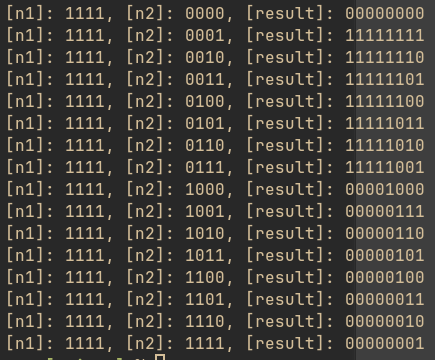
\includegraphics[width = 7cm]{426hw7log.png}
    \caption{Display log for ROM, \(n1 = -1\)}
    \label{fig:simlog}
\end{figure}

\textbf{Part B.}

This implementation already is pretty inefficient for two 4-bit numbers, so for two 8-bit numbers would be very tedious.

\smallskip

For a 4-bit 2's complement number system, you can represent -8 to 7. However, a 8-bit 2's complement number system can represent -128 to 127.

\smallskip

The case-statement method requires the engineer to individually compute the product magnitude for every single possibility, which for two 8-bit numbers would require 16 times more statements to complete as compared to the 4-bit implementation.

\smallskip

The problem statement does say for unsigned numbers, and this implementation is inefficient for both signed and unsigned numbers.

\end{document}
